\documentclass[a4paper,10pt]{article}
\topmargin-1cm
\addtolength{\textheight}{2.5cm}
\addtolength{\textwidth}{2cm}
\usepackage{times}

%Allow Colors
\usepackage[usenames, dvipsnames]{color}

\usepackage{verbatim}
\usepackage{graphicx}
\usepackage[german]{babel}
\usepackage[latin1]{inputenc}

\setlength{\parindent}{0cm}

\title{Latex Template}
\author{David Herzig}
\date{WS2004}

\begin{document}

HF-ICT - H"ohere Fachschule f"ur Informations- und Kommunikationstechnologie\\
CH 4132 Muttenz\\
P.S"utterlin

\vspace{2mm}

\begin{center}
{\Large \bf Vorkurs Informatik}\\
Exercise sheet 2 - 2018 Edition
\end{center}

\vspace{2mm}

\line(1,0){400}

\vspace{5mm}

\section{Gr"ossen der Informatik}

\begin{enumerate}

\item Auf Ihrer Festplatte befindet sich eine Datei \textbf{``foto.png''}. Im Eigenschaftenfenster der Datei sehen Sie, dass das File 18'220 Bytes an Nutzdaten umfasst - da Dateien aber immer aus einem oder mehreren Bl"ocken zu 4kB zusammengesetzt sind erscheint ausserdem eine separate Anzeige \textbf{``Gr"osse auf Datentr"ager''} ... d.h. der letzte Block wird von der Datei nicht immer vollst"andig belegt. \\
\\
Rechnen Sie aus:
% 18220 Bytes belegen 5 Bl"ocke zu 4096 Bytes - Ungenutzt um 5 Block sind (x = 18220 - 4 * 4096) 1836 Bytes
\begin{itemize}
\item Wieviele Bl"ocke die Datei belegen muss ? \\ \\
	 {\color{ForestGreen}
		 1 Block umfasst $4 \cdot 1024$ Bytes = 4'096 Bytes\\ \\
		 \underline{Ben"otigte Bl"ocke ermitteln:} \\ \\
		 $18220 \div 4096$ = 4 - Rest: 1836 \\ \\
		 4 ganze Bl"ocke + 1 Block der noch die restlichen Daten speichern muss. \\ \\
		 \textbf{5 Bl"ocke} insgesamt. \\
	 }
\item Wieviel Platz die zugewiesenen Bl"ocke effektiv auf dem Datentr"ager belegen ? \\ \\
	 {\color{ForestGreen}
		 5 Bl"ocke zu 4'096 Bytes belegen auf dem Datentr"ager 20'480 Bytes - d.h. genau 20kB.
	 }
\item Wieviele Bytes dabei ungenutzt bleiben ? \\ \\
	 {\color{ForestGreen}
		 Effektiv verbrauchter Platz 20'480 Bytes minus Nutzdaten 18'220 Bytes. \\ \\ 
		 \textbf{2'260 Bytes} verbleiben ungenutzt. \\
	 }
\end{itemize}

\item Wieviele bits werden ben"otigt, um die hexadezimale Zahl 88AA0244 zu speichern? \\
Wievielen Bytes entspricht das ? \\ \\ % 32 bit / 4 Bytes
	 {\color{ForestGreen}
	      Der maximale Wert einer einzelnen HEX Ziffer kann mit 4 bits dargestellt werden. \\ \\
		 D.h. die gegebene hexadezimale Zahl mit 8 Ziffern belegt $8 \cdot 4 = \mathbf{32}$ \textbf{bits}. \\ \\ 
		 Ein Byte umfasst 8 bits. \\ \\
		 $32$ bits $\div 8$ bits = \textbf{4 Bytes} werden ben"otigt. \\
	 }

\item Die Wellenform einer Musikdatei wird digital kodiert indem mehrere Amplitudenwerte einer Wellenform x mal in der Sekunde abgetastet werden. Der Wert der Amplitude wird mit einer Zahl fesgehalten - die Zahl kann dabei den Wert $0_{16}$ bis $FFFF_{16}$ annehmen - pro Sekunde der Aufzeichnung erfolgen 8000 Abtastungen (Aufl"osung = 8 kHz). Berechnen Sie nun die minimale "Ubertragungsrate (kbit/s) welche Ihr Internetprovider zur Verf"ugung stellen muss, damit ein Stereo Musikst"uck in Echtzeit "ubertragen werden kann (und zwar unkomprimiert) ? \\ \\
% Monodatenrate = 16 [bit] * 8000 [1/s] = 128kbit/s | Stereo = 256kbit/s
	 {\color{ForestGreen}
	      Eine einzelne Abtastung ben"otigt 16 bits. \\ \\
	      Pro Sekunde erfolgen 8000 Abtastungen - d.h. $16 bits \cdot 8000 [1/s] = 128000 [bits/s]$ \\ \\
	      Umgerechnet in kB pro Sekunde [kB/s] - $128000[bits/s] \div 1000 = 128[kbit/s]$ \\ \\
	      Um Stereo h"oren zu ko"nnen - d.h. 2 Kan"ale zu je 128[kbit/s] - muss die Datendurchsatzrate des Providers mindestens \textbf{256[kbit/s]} betragen.\\
	 }
	 
\vspace{3mm}

\begin{center}
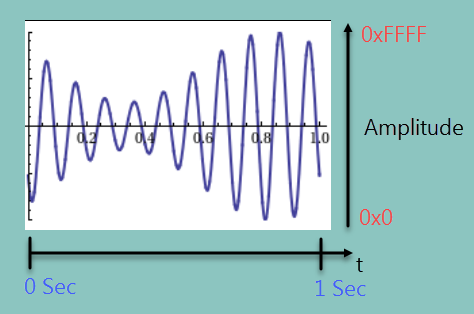
\includegraphics[width=150pt]{Wave.png}
\end{center}

\end{enumerate}

\section{ASCII Code}

\begin{enumerate}
\item "Ubersetzen Sie die Hexziffern in lesbaren ASCII Text.\\
\verb|42 52 41 56 4F 21| \\ \\ %BRAVO!
	 {\color{ForestGreen}
		 BRAVO \\
	 }

\item Wie lautet der Bin"arcode der ASCII Zeichenfolge ? \\
\verb|HF-ICT| \\ \\ %01001000 01000110 00101101 01001001 01000011 01010100
	 {\color{ForestGreen}
		 01001000 01000110 00101101 01001001 01000011 01010100 \\
	 }

\item "Ubersetzen Sie den folgenden ASCII Text.\\
\verb|01000001 01110010 01110100 01110111 01101111 01110010 01101011| \\ \\ %Artwork
	 {\color{ForestGreen}
		 Artwork \\
	 }
\end{enumerate}

\end{document}

